\documentclass[12pt, a4paper]{article}
\usepackage[utf8]{inputenc}
\usepackage[export]{adjustbox}
\usepackage{amsmath}
\usepackage{amsfonts}
\usepackage{amssymb}
\usepackage{xcolor}
\usepackage{graphicx}
\usepackage{subcaption}
\usepackage[left=2cm,right=2cm,top=2cm,bottom=2cm]{geometry}

\makeatletter
\renewcommand\thesubsection{\@arabic\c@subsection}
\makeatother

\newcommand{\figref}[1]{Figure~\ref{#1}}

\author{Maksym Polovyi}
\begin{document}

\subsection{}
\begin{figure*}[t]
\centering
	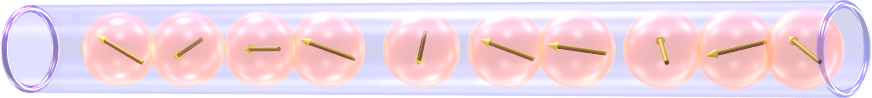
\includegraphics[width=0.9\textwidth]{Images/fullSystemPicture}
	\captionsetup{justification=centering, width=0.9\textwidth}
	\caption{Snapshot of system for density $\rho = 0.95$ and $k_BT = 1.5$. Arrows represent the dipole moment of the particle. System sample obtained by means of Langevin dynamics simulation. The simulation has run for $t = 100$, with fluid medium viscosity $\eta = 1$ and particle mass $m = 1$.}
	\label{fig:fullSystemPicture}
\end{figure*}

The phenomena under study is the existence of non-zero nematic order in a colloidal suspension consisting of short-rage interacting particles. As the model, we consider colloidal particles with a permanent dipole moment $\mu \hat{m}$, where $\hat{m}$ is a unitary vector with the direction of the dipole moment. While considering a three-dimensional system, we constrain particle translational motion to a one-dimensional line, i.e. particles are confined to the $z$ axis. However, particles can explore the full three dimensional orientation space. Example of particle positions and possible orientations after running a Langevin dynamics simulation is given at \figref{fig:fullSystemPicture}.

By constraining particles to a 1D tube we effectively enforce the direction of vector $\vec{r}_{ij}$ connecting particle centers to be co-aligned with $z$ axis. Assuming that all particles have the same dipole moment $\mu_i = \mu_j = \mu$, and defining $\mu = 1$ the energy of dipole-dipole interaction for any pair (i, j) of particles is given by:
\begin{equation}
\label{eq:dipole_dipole_1D}
E_{ij}^{dip} = - \epsilon \frac{1}{\Delta z^3} [3 \cos \theta_i \cos \theta_j - (\hat{m}_i \cdot \hat{m}_j)]
\end{equation}
where $\theta_i$ and $\theta_j$ are the angles between $z$ axis and dipole moments of the first and second particle respectively, and $\Delta z = |z_j - z_i|$, where $z_i$ and $z_j$ are particle positions along $z$ axis.

The repulsive part of particle-particle interaction is described by Yukawa potential
\begin{equation}
\label{eq:yukawa_interaction}
E_{ij}^{rep} = \epsilon \frac{A \exp(-k \Delta z)}{\Delta z}
\end{equation}
where $A$ and $k^{-1}$ --- are the strength and range of interaction.

In this study we concentrated on the values of $A = 1000$ and $k = 10$. \textcolor{red}{Add image of potential?}
Additionally, we restrict interaction to the immediate neighbors, and implement periodic boundary conditions.

\subsection{}
We measured the following quantities:

Nematic order parameter $S$ is defined as:
\begin{equation}
\label{eq:nematic_order_parameter}
	S = \frac{3 \langle\cos^2 \theta\rangle - 1}{2}
\end{equation}
where $\theta$ it the angle between particle dipole moment and spatial axis, while angle brackets denote ensemble average.
The nematic order for different values of $k_BT$, different densities and system sizes is shown on the Figure

We define particle $i$ to have Right orientation if angle $\theta_i$ is less than cut-off angle $\alpha = \pi/4$, Left orientation if $\theta_i > \pi - \alpha$, and Undefined orientation if $\alpha < \theta_i < \pi - \alpha$. 
Using this definitions, we measure the probability $P_{ij}$ of particles $i$ and $j = i+1$ have respectively Right-Right, Left-Left, Right-Left and Left-Right orientations.

For the study of time evolution of the system, we measure the auto-correlation function for \textcolor{red}{of} the orientation of a particle, defined as:
\begin{equation}
 \Phi(t) = \langle\Phi_i(t)\rangle = \langle\cos (\theta_i{m}) \cos (\theta_i)\rangle
\end{equation}
where angle brackets denote ensemble average.

\textcolor{red}{I can also do a better-looking distance-dependent correlation function}

\subsection{}

The time evolution of the system was studied by means of Langevin dynamics (LD) simulations, using the Velocity-Verlet integration scheme, while the equilibrium results were obtained by means of Monte-Carlo (MC) simulations, and later compared with long-time LD simulations.

The MC simulations were allowed to equilibrate for $\Delta = 5 \cdot 10^5$ sweeps (one sweep consists of $N$ Monte-Carlo test steps), and after that every $\Delta$ sweeps were generated ensemble-averaged quantities, obtaining that way $10$ uncorrelated samples. \textcolor{red}{Should I insert here the technical details about steps?}

As we can see on the \figref{fig:equilibrium_order_parameter}, the nematic order grows with the decrease of temperature, as well as with increase system density. The behaviour qualitatively doesn't changes for any of the observed density and $k_BT$. Non-zero values of nematic order parameter indicates that particles tends to co- or counter-align themselves with a selected axis and each other.

\begin{figure}
 \centering
 \begin{subfigure}{.45\textwidth}
  \centering
  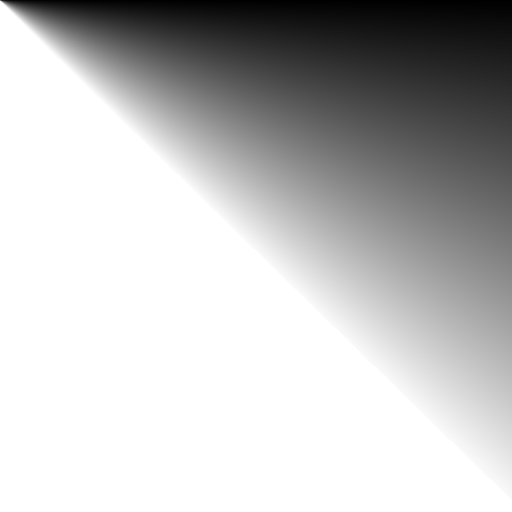
\includegraphics[width=0.8\textwidth]{Images/dummy.png}
 \end{subfigure}
 \begin{subfigure}{.45\textwidth}
  \centering
  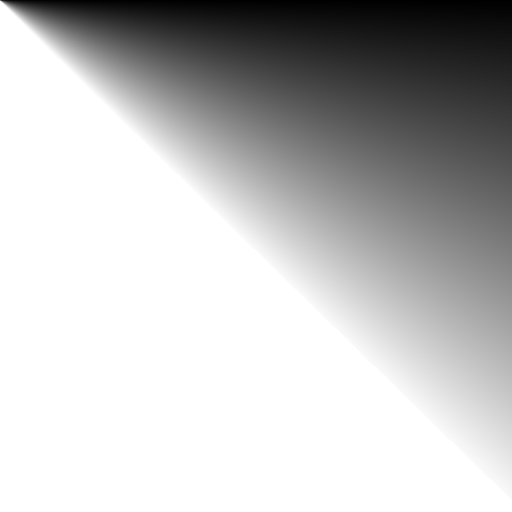
\includegraphics[width=.8\textwidth]{Images/dummy.png}
 \end{subfigure}
 \captionsetup{justification=centering, width=0.9\columnwidth}
 \caption{Nematic order as function of $k_BT$ for different densities and system sizes (left). As function of density for different $k_BT$ and system sizes (right) \textcolor{red}{I'll place real pictures when I'll get to work}}
 \label{fig:equilibrium_order_parameter}
\end{figure}

The equilibrium probabilities for two particles have same or opposite direction (as defined above) are shown at the \figref{fig:equilibrium_orientation_prob}. As expected, the probability of two particle being co-aligned with each other is higher that to be counter-aligned. What is important to mention, however, is that probabilities of Left-Left and Right-Right configurations are the same, meaning that orientation along and against the spatial axis are indistinguishable.

\begin{figure}
 \centering
 \begin{subfigure}{.45\textwidth}
  \centering
  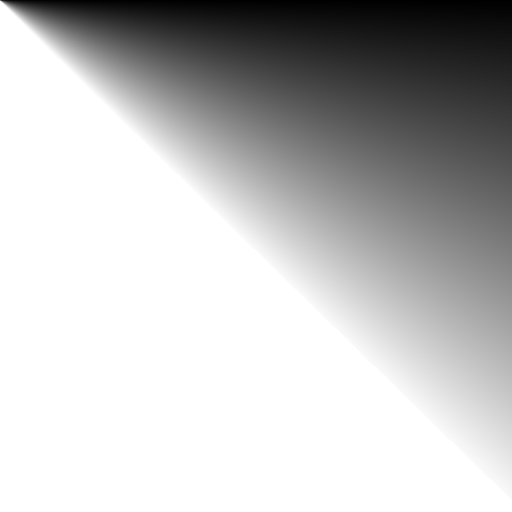
\includegraphics[width=0.8\textwidth]{Images/dummy.png}
 \end{subfigure}
 \begin{subfigure}{.45\textwidth}
  \centering
  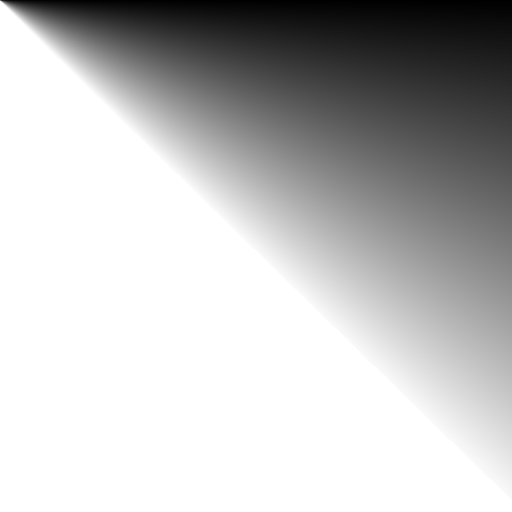
\includegraphics[width=.8\textwidth]{Images/dummy.png}
 \end{subfigure}
 \captionsetup{justification=centering, width=0.9\columnwidth}
 \caption{Particle pairs orientation probabilities as function of $k_BT$ for different system sizes with fixed density $\rho = 0.5$ (left). As function of density for different system sizes with fixed $\k_BT = 1$ (right) \textcolor{red}{I'll place real pictures when I'll get to work}}
 \label{fig:equilibrium_orientation_prob}
\end{figure}

The \figref{fig:equilibrium_orientation_prob} shows the relaxation of order parameter to an equilibrium value for different densities and temperatures. As we can see, even for low temperature (and high values of order parameter) the decay is exponential. The molecular dynamics relax 

\begin{figure}
 \centering
 \begin{subfigure}{.45\textwidth}
  \centering
  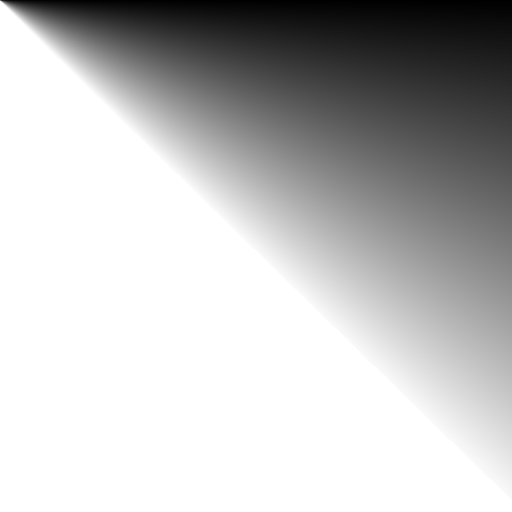
\includegraphics[width=0.8\textwidth]{Images/dummy.png}
 \end{subfigure}
 \begin{subfigure}{.45\textwidth}
  \centering
  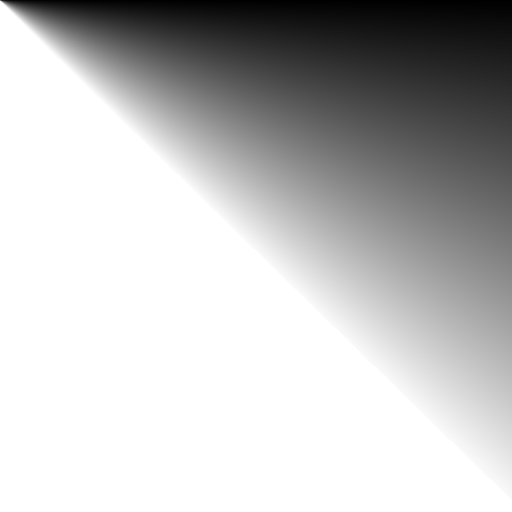
\includegraphics[width=.8\textwidth]{Images/dummy.png}
 \end{subfigure}
 \captionsetup{justification=centering, width=0.9\columnwidth}
 \caption{Approaching of the system order parameter to the equilibrium values for different densities and temperatures. The results are averaged over $100$ samples of $3200$ particles.  \textcolor{red}{I'll place real pictures when I'll get to work}}
 \label{fig:equilibrium_orientation_prob}
\end{figure}b

\end{document}